\section{Prototypen}
Im Rahmen der Entwicklung des finalen Endprogramms wurden mehrere Prototypen entwickelt um sich erstens in die einzelnen SDKs einzuarbeiten und zweitens die Prototypen zu erweitern und zu vereinen. Diese Prototypen werden hier vorgestellt.

\subsection{Erster Kinect-Prototyp}
Anhand der obigen Überlegungen wurde der erdachte Algorithmus zunächst anhand eines Prototyps implementiert. Dieser sollte zunächst dazu dienen, das Microsoft Kinect SDK näher kennen zu lernen\todo{getrennt zusammen?}. Der erste Prototyp erfüllte folgende Funktionen:\\
-Kinect SDK Library
-(Connect-Disconnect von Kinect)
-Winkelerkennung des Benutzers mit Anzeige in Grad
-Anzeige des Kamerabildes mit Gelenkkennzeichnung von Kopf und Armen
\todo{Bild}

\subsection{Erster Nao-Prototyp}
Zur Einarbeitung in das Nao-SDK wurde eine Anwendung erstellt, die verschiedene Armwinkel an den Roboter übermitteln können.

In Bild \myref{f:nao_prototyp1} sind verschiedene Eingabefelder zu sehen. In die oberste wird die IP - Adresse eingetragen, die dem zu benutzenden Nao (hier: lokal in Webots) entspricht. Bei einem Klick auf den Button \textit{Connect} wird im Hintergrund ein neuer Proxy geöffnet. Wenn die Verbindung erfolgreich aufgebaut wurde, wird auch der Button \textit{Move} klickbar.
\begin{figure}[H]						
	\centering							
	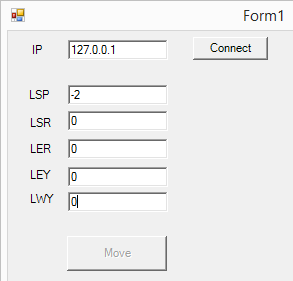
\includegraphics[scale=0.8]{Bilder/nao_prototyp1.PNG}
	\caption{Erster Nao-Prototyp}						
	\label{f:nao_prototyp1}						
\end{figure}
In die anderen Felder müssen die einzelnen Winkel (im Bogenmaß) für die Gelenke (LSP = LeftShoulderPitch, LSR = LeftShoulderRoll, usw.) eingetragen werden. Bei Klick auf den Button \textit{Move} werden die einzelnen Winkel des linken Arms in die Position der eingetragenen Werte gefahren. In diesem Fall hebt der Roboter den linken Arm nach oben an, da \textit{LSP} mit -2rad definiert ist und dies im Nao - Gelenkraum einem Winkel von $-115^{\circ}$ entspricht (siehe Kapitel \ref{tab:Lgelenkraum} und Bild \ref{f:gelenkraumL}). 

Ist ein angegebener Winkel nicht im Gelenkbereich wird die komplette Bewegung nicht ausgeführt. (gilt nur für diesen Prototyp)

\subsection{Zweiter Prototyp}
Anhand der ersten Prototypen wurde das nun erworbene Wissen in eine gemeinsame Architektur eingebettet (Siehe Kapitel Architektur). Als Verbesserungen wurden alle benötigten Winkel auf zwei separaten Fenstern angezeigt, eines für jeden Arm. Auf der GUI wird nun das komplette Skelett über das RGB-Bild gelegt.
\todo{Screenshot}


\subsection{Endprogramm}
Um den effektiven Algorithmus der Winkelerkennung noch effizienter zu gestalten wurde noch ein Mittelwertsfilter implementiert, um die Ausreißer in den erkannten Winkeln zu eliminieren und somit die Messungenauigkeit der Gelenkpositionen zu verringern.


\todo{Screenshot von Prototypprogramm}